\documentclass{article}
\usepackage[T1]{fontenc}
\usepackage{lmodern}
\usepackage{graphicx}
\usepackage{amsmath,amssymb}
\usepackage[a4paper,margin=2cm]{geometry}
\usepackage[absolute,overlay]{textpos}
\setlength{\TPHorizModule}{1mm}
\setlength{\TPVertModule}{1mm}
\usepackage[indonesian]{babel}
\usepackage{hyperref}
\setlength{\emergencystretch}{2em}
% unit: Halaman 3

\begin{document}

% === Halaman 3 (llm) ===

\begin{itemize}
  \item \textit{Cipher} di dalam kriptografi klasik disusun oleh dua teknik dasar:
  \begin{enumerate}
    \item \textbf{Teknik substitusi}: mengganti huruf plainteks dengan huruf cipherteks.
  \end{enumerate}
\end{itemize}

\vspace{10mm}

\begin{itemize}
  \item[] Contoh: \quad Plainteks: \texttt{MENGANTUK} \\ Cipherteks: \texttt{CQBSIBONW}
\end{itemize}

\vspace{10mm}

\begin{enumerate}
  \setcounter{enumi}{1}
  \item \textbf{Teknik transposisi}: mengubah susunan atau posisi huruf plainteks menjadi susunan huruf cipherteks. \\ Disebut juga teknik \textit{scrambling}, permutasi, atau pengacakan \\ Contoh: \quad Plainteks: \texttt{MENGANTUK} \\ Cipherteks: \texttt{TNEAKMNGU}
\end{enumerate}

% deskripsi: Tabel pemetaan substitusi huruf alfabet dari Plainteks ke Cipherteks
% bbox normalisasi: [0.1350, 0.2370, 0.9500, 0.3480]
\begin{textblock*}{171.15mm}(28.35mm,70.39mm)
\noindent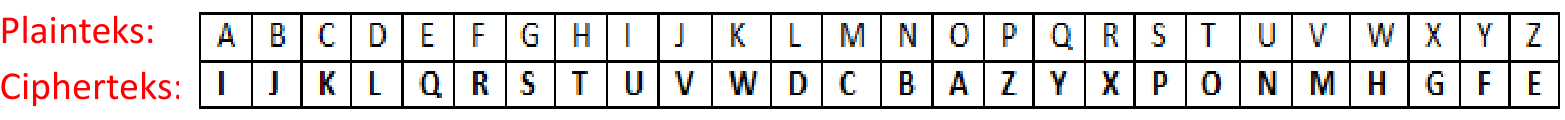
\includegraphics[width=171.15mm,height=32.97mm]{../../images/llm/page_003_img_01.png}%
\end{textblock*}

\end{document}
